\newpage
\section{Utilities}
\label{sec:utilities}

\begin{description}

%------------------------------------------------------------------------------
\addcontentsline{toc}{subsection}{btkApplyMaskToImage}
\item[btkApplyMaskToImage]: Mask an image with a mask (ITK filter: MaskImageFilter).
%------------------------------------------------------------------------------
\addcontentsline{toc}{subsection}{btkAverage3DImages}
\item[btkAverage3DImages]: Compute the mean (and variance) image of a set of 3D images.
%------------------------------------------------------------------------------
\addcontentsline{toc}{subsection}{btkAverageImagesWithReference}
\item[btkAverageImagesWithReference]: ?
%------------------------------------------------------------------------------
\addcontentsline{toc}{subsection}{btkBinarizeLabels}
\item[btkBinarizeLabels]: Binarize one label image (depending on the label value chosen).
%------------------------------------------------------------------------------
\addcontentsline{toc}{subsection}{btkBinarizeMask}
\item[btkBinarizeMask]: Binarize a float image using a threshold.
%------------------------------------------------------------------------------
\addcontentsline{toc}{subsection}{btkBinarizeTissueProbabilityMaps}
\item[btkBinarizeTissueProbabilityMaps]: Binarize a set of probability maps ([0,1]) into a short image (by taking the max probability at each voxel). (pourquoi ne pas faire un truc generique?)
%------------------------------------------------------------------------------
\addcontentsline{toc}{subsection}{btkComputeChamferDistance}
\item[btkComputeChamferDistance]: Compute the chamfer distance.
%------------------------------------------------------------------------------
\addcontentsline{toc}{subsection}{btkComputeOverlap}
\item[btkComputeOverlap]: Compute the overlap (Dice coefficient and Jaccard index) between two label images.
%------------------------------------------------------------------------------
\addcontentsline{toc}{subsection}{btkConvertGradientTable}
\item[btkConvertGradientTable]: Transform gradients from world to image coordinates.

%------------------------------------------------------------------------------
\addcontentsline{toc}{subsection}{btkCropImageUsingMask}
\item[btkCropImageUsingMask] This program crops one (3D or 4D) image using a 3D mask.
%------------------------------------------------------------------------------
\addcontentsline{toc}{subsection}{btkDifferentialBiasCorrection}
\item[btkDifferentialBiasCorrection]: Differential bias correction method for $n$ images (Leung et al. Neuroimage 2012) 

%------------------------------------------------------------------------------
\addcontentsline{toc}{subsection}{btkDistanceBetweenBinaryImages}
\item[btkDistanceBetweenBinaryImages]: Compute Hausdorff and Mean Contour Distances between two binary images (ITK Filters: HausdorffDistanceImageFilter and ContourMeanDistanceImageFilter).
%------------------------------------------------------------------------------
\addcontentsline{toc}{subsection}{btkExtractMaskUsingBoundingBox}
\item[btkExtractMaskUsingBoundingBox]: Extract Masks using the intersection of the bounding boxes of images.
%------------------------------------------------------------------------------
\addcontentsline{toc}{subsection}{btkExtractOneImageFromSequence}
\item[btkExtractOneImageFromSequence] This program extracts one image from a 4D sequence. It can be useful for diffusion MRI image analysis. 
%------------------------------------------------------------------------------
\addcontentsline{toc}{subsection}{btkFCMClassification}
\item[btkFCMClassification]: Fuzzy C-means classification algorithm.
%------------------------------------------------------------------------------
\addcontentsline{toc}{subsection}{btkHistogramMatching}
\item[btkHistogramMatching]: Normalize the grayscale values of one image using a reference image by histogram matching (ITK filter: HistogramMatchingImageFilter).%------------------------------------------------------------------------------
\addcontentsline{toc}{subsection}{btkImageGaussianFilter}
\item[btkImageGaussianFilter]: Apply a gaussian filter on an image (ITK filter: DiscreteGaussianImageFilter).
%------------------------------------------------------------------------------
\addcontentsline{toc}{subsection}{btkImageHistogram}
\item[btkImageHistogram]: Analysis of images through histograms (It can save into text files histogram, cumulative distribution function (cdf) and inverse-cdf of an image).
%------------------------------------------------------------------------------
\addcontentsline{toc}{subsection}{btkImageInjection}
\item[btkImageInjection] This program performs the injection of a set
of images with an already existing set of transformations. This avoids the need
to perform a new image reconstruction (computationally expensive) after
modification of the input images (some filtering for example) or an involuntary
deletion of the reconstructed image.

Recommended usage: \texttt{btkImageInjection -i image1 $\cdots$ -i
imageN -m mask1 $\cdots$ -m maskN -t transform1 $\cdots$ -t
transformN -o output --mask}

%------------------------------------------------------------------------------
\addcontentsline{toc}{subsection}{btkImageMorphologicalClosing}
\item[btkImageMorphologicalClosing]: Greyscale Morphological Closing by a ball structuring element (ITK filter: GrayscaleMorphologicalClosingImageFilter).
%------------------------------------------------------------------------------
\addcontentsline{toc}{subsection}{btkImageMorphologicalTopHat}
\item[btkImageMorphologicalTopHat]: Greyscale Morphological Top Hat by a ball structuring element.
%------------------------------------------------------------------------------
\addcontentsline{toc}{subsection}{btkImageResampling}
\item[btkImageResampling]: Resample an image using: 1) a reference image (better option) or 2) specific size or spacing (mainly based on ITK filter: ResampleImageFilter)
%------------------------------------------------------------------------------
\addcontentsline{toc}{subsection}{btkImageSimilarity}
\item[btkImageSimilarity]: Calculates mean square error, mutual information, normalized correlation and normalized mutual information of two images A and B. The use of a mask is possible.
%------------------------------------------------------------------------------
\addcontentsline{toc}{subsection}{btkImageSubtract}
\item[btkImageSubtract]: Pixel-wise subtraction of two image, or one image and a constant (-i im1 -i im2 -o result or -i im1 -c value -o result) (ITK filter: SubtractImageFilter).
%------------------------------------------------------------------------------
\addcontentsline{toc}{subsection}{btkIteratedBackProjection}
\item[btkIteratedBackProjection]: Apply iterated back projection to high resolution image using one low resolution image.
%------------------------------------------------------------------------------
\addcontentsline{toc}{subsection}{btkMajorityVoting}
\item[btkMajorityVoting]: Compute label map using majority voting rule.
%------------------------------------------------------------------------------
\addcontentsline{toc}{subsection}{btkMidwayHistogramEqualization}
\item[btkMidwayHistogramEqualization]: Perform midway histogram equalization for a set of 3D images (cf Delon JMIV 2004).
%------------------------------------------------------------------------------
\addcontentsline{toc}{subsection}{btkModifyImageUsingLookUpTable}
\item[btkModifyImageUsingLookUpTable] This program modifies one image using a
look up table defined in a ascii file (2 columns, one for the original values,
one for the final values). It can be useful to relabel a segmented image. 

%------------------------------------------------------------------------------
\addcontentsline{toc}{subsection}{btkNiftiToNrrd}
\item[btkNiftiToNrrd] This program convert a diffusion sequence in nifti
format\footnote{Currently there is no nifti standard for DWI, so DW images are
saved as a standard nifti sequence (*.nii, *.nii.gz) and two text files
containing the b-values (.bval) and the gradient directions (.bvec).}  to the
nrrd format (*.nhdr). Usage: \texttt{-i input -o output.nhdr}

%------------------------------------------------------------------------------
\addcontentsline{toc}{subsection}{btkNrrdToNifti}
\item[btkNrrdToNifti] This program convert an image from Nrrd file (*.nhdr and *.nrrd) to a Nifti file (*.nii or *.nii.gz). The conversion of a DWI image is possible by using the option \texttt{--dwi}. Usage: \texttt{-i input.nhdr -o output.nii.gz}. Usage for DWI sequence: \texttt{--dwi -i input.nhdr -o output.nii.gz}.
%------------------------------------------------------------------------------
\addcontentsline{toc}{subsection}{btkPrintImageInfo}
\item[btkPrintImageInfo]: Prints image information (size, origin, spacing, directions, anatomical orientation, pixel type).
%------------------------------------------------------------------------------
\addcontentsline{toc}{subsection}{btkProbabilityMapNormalization}
\item[btkProbabilityMapNormalization]: Normalize in a voxelwise manner a set of (positive) probability maps. 
%------------------------------------------------------------------------------
\addcontentsline{toc}{subsection}{btkPSNR}
\item[btkPSNR]: Compute the PSNR between an input image and a reference image.
%------------------------------------------------------------------------------
\addcontentsline{toc}{subsection}{btkReconstructionComparisonTool}
\item[btkReconstructionComparisonTool]: Compare several reconstruction methods: creates a label image explaining which reconstructed image is the best at each voxel.
%------------------------------------------------------------------------------
\addcontentsline{toc}{subsection}{btkRegisterDiffusionToAnatomicalData}
\item[btkRegisterDiffusionToAnatomicalData] This program registers a DW
sequence to an anatomical image. 

%------------------------------------------------------------------------------
\addcontentsline{toc}{subsection}{btkReorientDiffusionSequenceToStandard}
\item[btkReorientDiffusionSequenceToStandard] Reorients a DW sequence
to the standard orientation. This is necessary with fetal images since the fetus
is in a random orientation with respect to the scanner. This is particularly
important in DWI because colormaps lack of significance, which makes difficult
the identification of specific bundles.

Usage: \texttt{btkReorientDiffusionSequenceToStandard -i image -o output -l
landmarks}.

\texttt{landmarks} is a landmarks file obtained as explained for btkReorientImageToStandard.

%------------------------------------------------------------------------------
\addcontentsline{toc}{subsection}{btkReorientImageToStandard}
\item[btkReorientImageToStandard] This program reorients a image to the standard orientation. This is necessary with fetal images since in general the fetus is in a random orientation with respect to the scanner.
Usage: \texttt{btkReorientImageToStandard -i image -o output -l landmarks}.
\texttt{landmarks} is a text file containing points that define the left-right
and the posterior-anterior directions. The points $l$ and $r$ define the left
$\rightarrow$ right direction, and the points $p$ and $a$ define the posterior
$\rightarrow$ anterior direction. Such file can be easily generated by using
\href{http://www.slicer.org}{Slicer} (version 3) as follows:

\begin{enumerate}
\item Open the high-resolution image by using the \textit{Volume} module.
\item Toogle on the visibility of all slices in the 3D view. This allows to
identify the left and right sides of the brain in the 2D views.
\item Place the landmarks $l$, $r$, $p$, and $a$ in this order by using
\texttt{[p]}.
\item Save the file (*.fcsv) by using the menu File $\rightarrow$ Save.
\end{enumerate}


\begin{figure}[t]
\centering
\begin{tabular}{ccc}
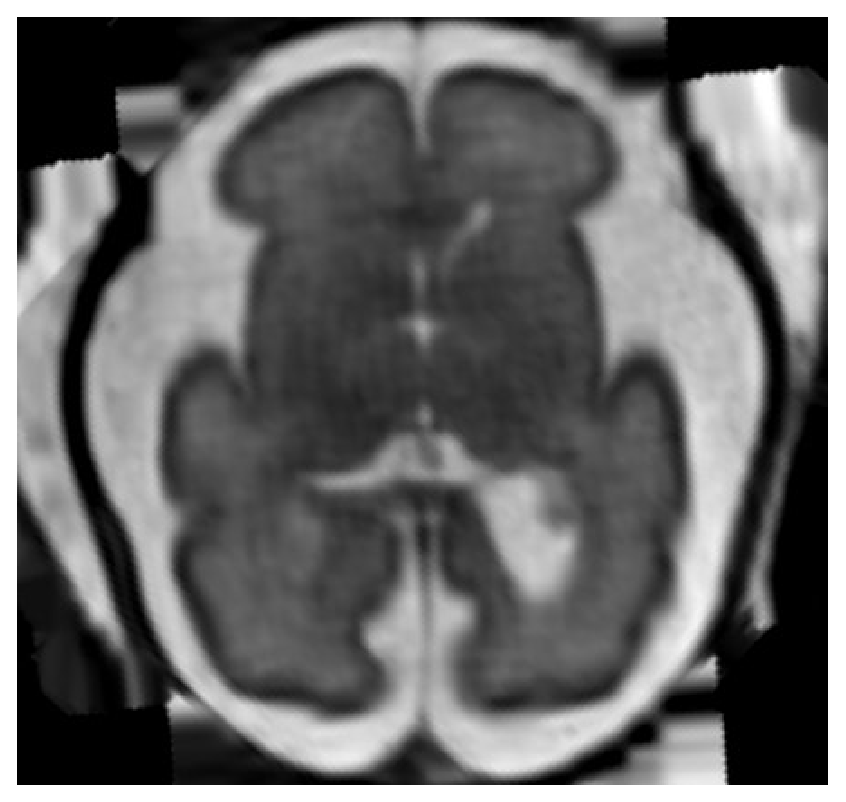
\includegraphics[width=0.3\columnwidth]{hr_axl.eps}&
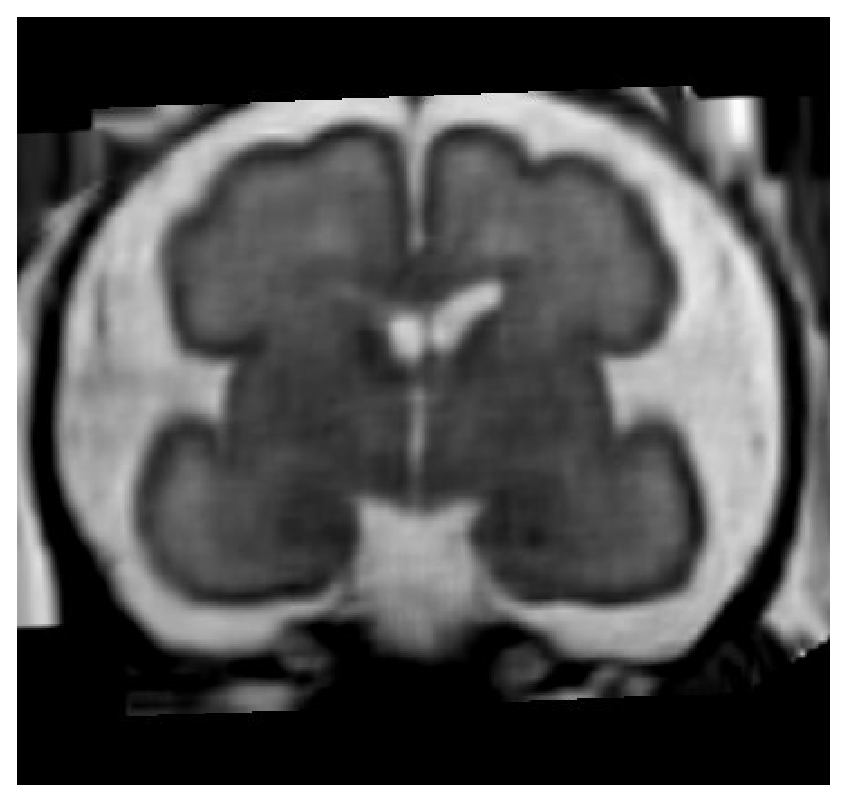
\includegraphics[width=0.3\columnwidth]{hr_cor.eps}&
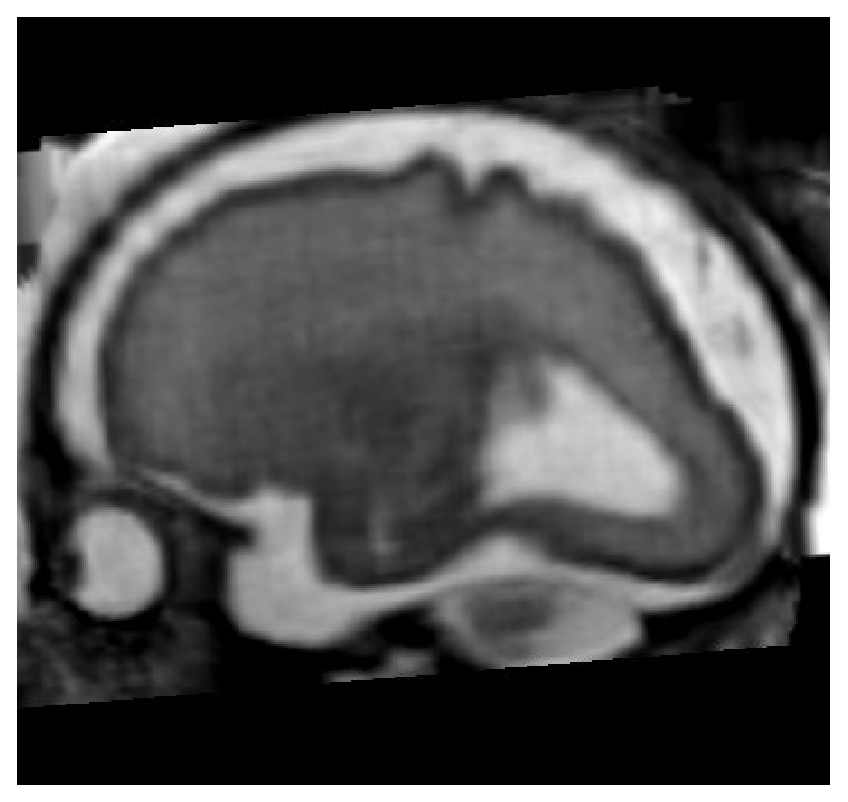
\includegraphics[width=0.3\columnwidth]{hr_sag.eps}\\
{(a)}&{(b)}&{(c)}\\
\end{tabular}
\caption{Example of an anatomical reconstruction of a fetal brain by using
\texttt{btkImageReconstruction}. (a) axial, (b) coronal, and (c) sagital view.}
\label{fig:reconstruction}
\end{figure}

\begin{figure}[t]
\centering
\begin{tabular}{cc}
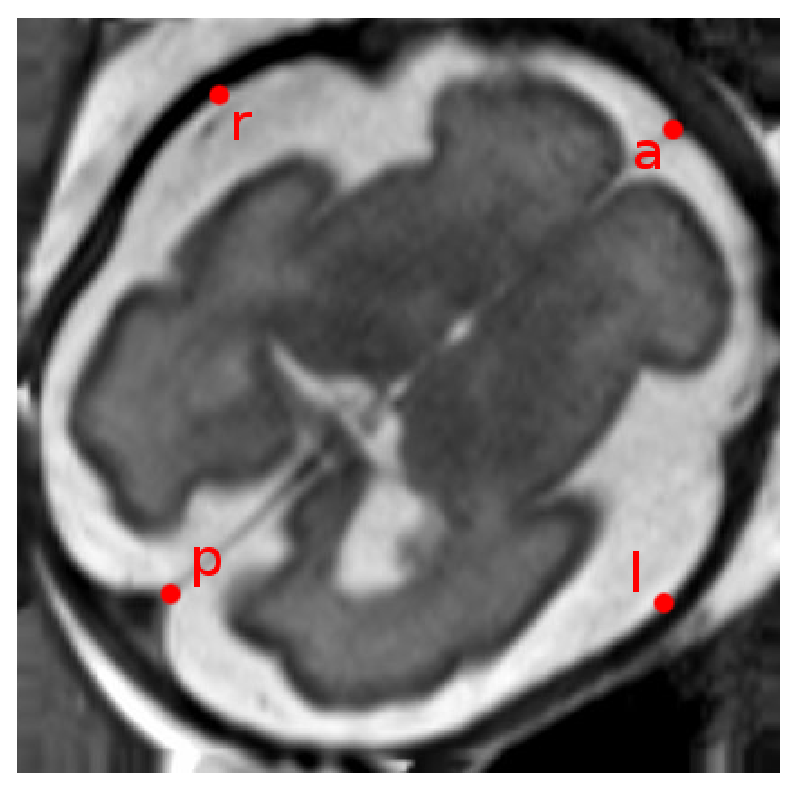
\includegraphics[width=0.35\columnwidth]{lmks_axial.eps}&
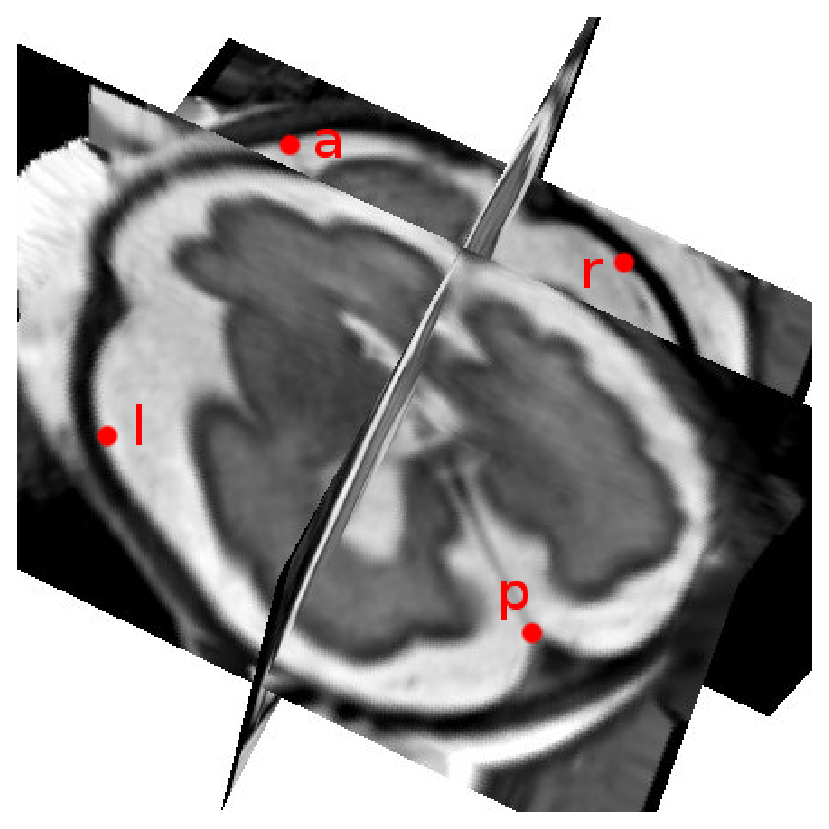
\includegraphics[width=0.35\columnwidth]{lmks_3D.eps}\\
{(a)}&{(b)}\\
\end{tabular}
\caption{Placement of landmarks by using Slicer. (a) axial slice, (b) 3D view.}
\label{fig:landmarks}
\end{figure}

%------------------------------------------------------------------------------
\addcontentsline{toc}{subsection}{btkResampleLabelsByInjection}
\item[btkResampleLabelsByInjection]: Resample a set of label images using the injection method.
%------------------------------------------------------------------------------
\addcontentsline{toc}{subsection}{btkRescaleIntensity}
\item[btkRescaleIntensity]: Rescale the intensity values of an image using short values (possibility to use a mask image).
%------------------------------------------------------------------------------
\addcontentsline{toc}{subsection}{btkSequenceNormalization}
\item[btkSequenceNormalization]: Writes a dwi sequence as a single image B0 + the diffusion images. The new B0 is the mean of all B0 images in the original sequence, or a user-provided B0.
%------------------------------------------------------------------------------
\addcontentsline{toc}{subsection}{btkSetStandardCoorSystem}
\item[btkSetStandardCoorSystem]: Sets the direction to the identity, and the origin to the center of the image.
%------------------------------------------------------------------------------
\addcontentsline{toc}{subsection}{btkSimulateMotionSliceBySlice}
\item[btkSimulateMotionSliceBySlice]: Apply transformations on slices of input image.
%------------------------------------------------------------------------------
\addcontentsline{toc}{subsection}{btkSimulateStandardViewFromIsotropicImage}
\item[btkSimulateStandardViewFromIsotropicImage]: Simulates standard acquisitions (axial, coronal, and sagital) from an isovoxel by using an observational model. This is useful for example to assess the performance of reconstruction algorithms according to the subsampling factor (the reconstructed image from the simulated images is then compared to the isovoxel image). 
%------------------------------------------------------------------------------
\addcontentsline{toc}{subsection}{btkTranslateImageOverTemplate}
\item[btkTranslateImageOverTemplate]: Usefull for the extraction mask pipeline, it will translate the center of image (or barycenter of masked image) on the center of the template image.
%------------------------------------------------------------------------------
\addcontentsline{toc}{subsection}{btkWarpTransformationToImage}
\item[btkWarpTransformationToImage]: Apply a itk or btk transformation on a image.
%------------------------------------------------------------------------------
\addcontentsline{toc}{subsection}{btkWeightedSum}
\item[btkWeightedMean]: Compute a weighted mean of 3D images (no check for normalized weights!).
%------------------------------------------------------------------------------
\addcontentsline{toc}{subsection}{btkWeightedSumOfAffineTransforms}
\item[btkWeightedSumOfAffineTransforms]: Compute a weighted mean of affine transforms (no check for normalized weights!).
%------------------------------------------------------------------------------



\end{description}
